\documentclass[10pt,xcolor=pdflatex]{beamer}
\usepackage{newcent}
\usepackage[utf8]{inputenc}
%\usepackage[czech]{babel}
\usepackage{hyperref}
\usepackage{fancyvrb}
\usepackage{multicol}

\usetheme{FIT}

%%%%%%%%%%%%%%%%%%%%%%%%%%%%%%%%%%%%%%%%%%%%%%%%%%%%%%%%%%%%%%%%%%
\title{Continuous Integration and Automated Code Review in Open Source Projects}

\author[]{Adrián Tóth}

\institute[]{
    Brno University of Technology, Faculty of Information Technology\\
    Bo\v{z}et\v{e}chova 1/2. 612 66 Brno - Kr\'alovo Pole\\
    xtotha01@fit.vutbr.cz
    }

%\date{January 1, 2016}
%\date{\today}
\date{} % bez data

%%%%%%%%%%%%%%%%%%%%%%%%%%%%%%%%%%%%%%%%%%%%%%%%%%%%%%%%%%%%%%%%%%

\begin{document}

% 1
\frame[plain]{\titlepage}

% 2
\begin{frame}\frametitle{Introduction}
    \begin{center}
        \begin{tabular}{l}
            Continuous Integration \& Automated Code Review\\[1em]
            Red Hat, Inc. \& ManageIQ\\[1em]
            ManageIQ Bot
        \end{tabular}
    \end{center}
\end{frame}

% 3
\begin{frame}\frametitle{Components of CI System}
    \begin{figure}[H]
        \centering
        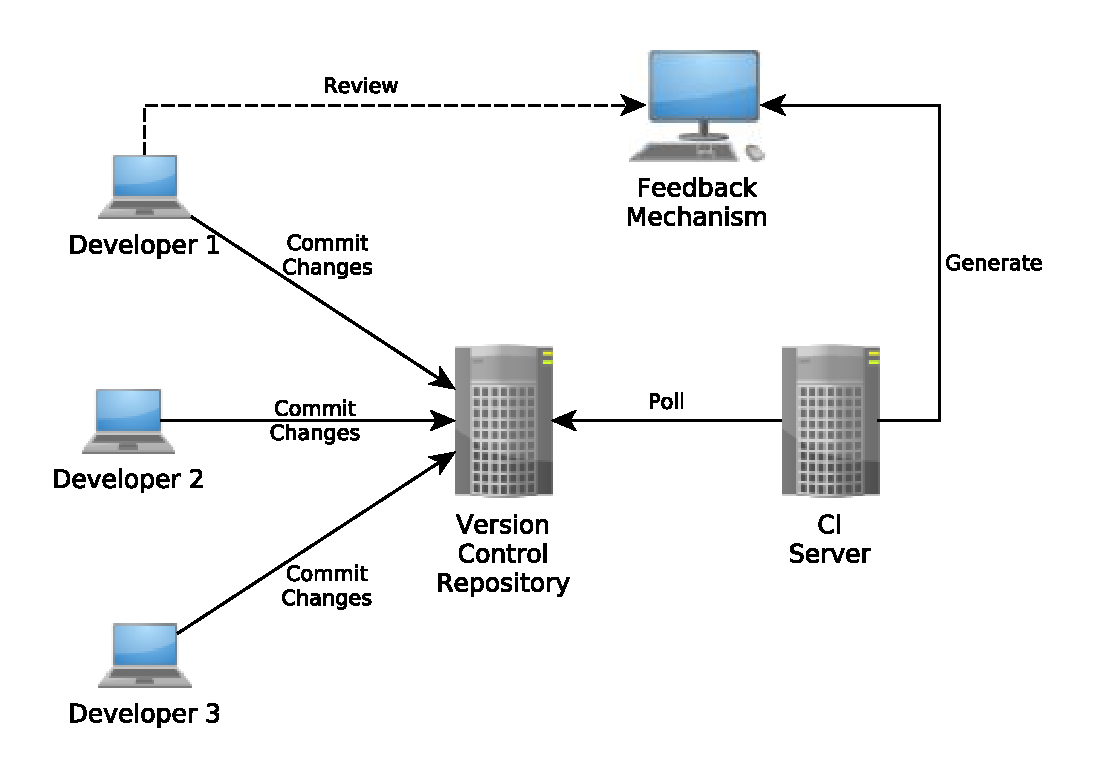
\includegraphics[scale=0.5]{eps/components_of_CI_system.eps}
    \end{figure}
\end{frame}

% 4
\begin{frame}\frametitle{ManageIQ Bot}
    \begin{itemize}
        \item Ruby 2.3.6\\[1em]
        \item Sidekiq
            \begin{itemize}
                \item background processing for Ruby
                \item nonrecurring \& recurring workers\\[1em]
            \end{itemize}
        \item Octokit
            \begin{itemize}
                \item Ruby toolkit for the GitHub API\\[1em]
            \end{itemize}
        \item Redis \& PostgreSQL
    \end{itemize}
\end{frame}

% 5
\begin{frame}\frametitle{Objectives}
    \begin{itemize}
        \item \textit{Pronto}\footnotemark \ integration\\[0.5em]
        \item MiqBot's own \textit{Pronto}\footnotemark[\value{footnote}] Formatter\\[0.5em]

        \footnotetext{\color{cyan}\href{https://github.com/prontolabs/pronto}{github.com/prontolabs/pronto}} 

        \item \textit{Gitter}\footnote{\color{cyan}\href{https://github.com/kristenmills/ruby-gitter}{github.com/kristenmills/ruby-gitter}} integration (yell if master is broken)\\[0.5em]
        \item \textit{Github Status API}\footnote{\color{cyan}\href{https://developer.github.com/v3/repos/statuses}{developer.github.com/v3/repos/statuses}} integration\\[0.5em]
        \item Remove unnecessary unmergeable comments
        \item Commands\\
            \begin{itemize}
                \item pull request review request from specified user(s)
                \item remove pull request review request from specified user(s)
                \item remove assigned user(s)
            \end{itemize}
        \item Automated review request of a new pull request
    \end{itemize}
\end{frame}

% 6
\begin{frame}\frametitle{Pronto Integration}
\end{frame}

% 7
\begin{frame}\frametitle{Gitter Integration}
\end{frame}

% 8
\begin{frame}\frametitle{GitHub Status API Integration}
\end{frame}

% 9
\begin{frame}\frametitle{Interface Commands}
\end{frame}

% 11
\bluepage{Thank You For Your Attention !}

\end{document}
